\chapter{Processo de Jogos Eletrônicos Com Monitoramento de Dados de Saúde}

Para a elaboração deste processo foi realizada uma revisão da literatura sobre desenvolvimento de jogos tradicionais (Capítulo \ref{cap:desenvolvimento_jogos}) ~\cite{keith2010agile,moore2011basics,rucker2003,kanode2009} software e das necessidades encontradas no desenvolvimento de jogos voltados para saúde como ~\cite{Suhonen_2010,herber2011,bartolome11,sinclair07,Hardy2011,kato12}. O objetivo deste trabalho definir a possibilidade sobre o desenvolvimento de um jogo para entretenimento que permita o monitoramento de dados de saúde de modo não invasivo e não se preocupa com os problemas de criar um \texit{game design} atrativo e envolvente.

%Para a elaboração desse processo foram utilizados estudos empíricos através de técnicas de pesquisa qualitativa com o uso de entrevista semi-estruturada \cite{FLI04} e observação participativa em um estudo de caso \cite{Yin05}. O resultado dessas avaliações estã descritos na \secref{section:analise_entrevista_semi_estruturada}. Como resultado dessa análise foram extraídos requisitos (\secref{section:requisitos_entrevista} e \secref{section:requisitos_estudo_caso}) que definiram algumas características e problemas de ambientes distribuídos de desenvolvimento, os quais requerem maior atenção em relação ao desenvolvimento presencial, como: uso de ferramentas colaborativas, meios de comunicação e coordenação das equipes distribuídas. 

Como procuramos propor um processo completo para ser customizado a toda e qualquer aplicação, é importante que a equipe de desenvolvimento faça uma análise inicial do processo como um todo e de acordo com suas necessidades avalie que atividades e artefatos devem ser instanciados para o projeto.

A modelagem deste processo fez uso da semântica do meta-modelo \ac{spem} na Versão 2.0 \cite{spem08} que permite modelar métodos, atividades de processos de software através da notação gráfica UML. O SPEM 2.0 é usado para definir processos de desenvolvimento de software, sistemas e seus respectivos componentes. O escopo da SPEM se restringe aos elementos necessários para definir qualquer processo de desenvolvimento de software, sem adicionar funcionalidades específicas para domínios particulares (como por exemplo, desenvolvimento de um jogo). Como pode ser visto na Figura \ref{fig:spem20}, o meta-modelo está estruturado em sete pacotes de meta-modelos. A estrutura divide o modelo em unidades lógicas com responsabilidades bem definidas e cada unidade compartilha informações gerando dependências entre elas sendo capaz de suportar diferentes variedades de ciclo de vida, como: em cascata, iterativo e incremental, evolucionário e assim por diante.

\begin{figure}
 \centering
 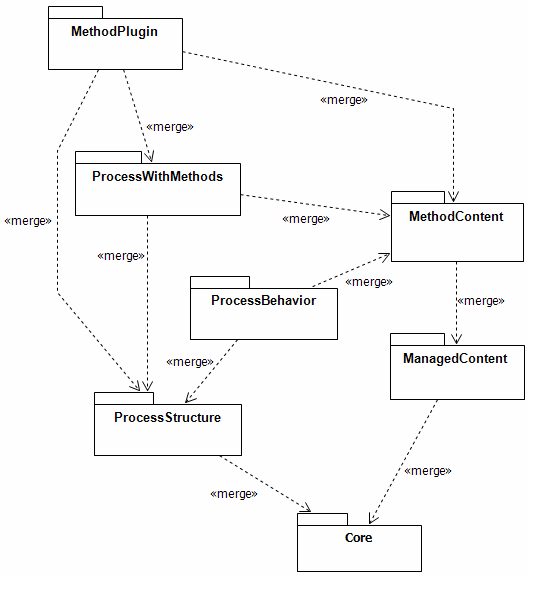
\includegraphics[scale=0.5]{./img/spem20.png}
 % matrixargseg.png: 296x162 pixel, 100dpi, 7.52x4.11 cm, bb=0 0 213 117
 %\caption{Estágio desenvolvimento de jogos ~\cite{fullerton2008game}}
\caption{Estrutura do meta-modelo SPEM 2.0}
%  \caption{Estágio desenvolvimento de jogos}
 \label{fig:spem20}
\end{figure}

Esse processo foi modelado a partir da ferramenta \ac{epf} \cite{epf13}, essa ferramenta é utilizada para autoria de processos através da notação de descrição de processos \ac{spem} \cite{spem08}. A partir dela é possível criar, customizar e publicar os processos de desenvolvimento.

\section{Visão Geral}
O processo proposto, chamado GAme Health Monitor Embedded-UFCG Process (\textit{GAHME Process}), aborda o desenvolvimento de jogos, com o objetivo monitorar dados de saúde por intermédio de jogos eletrônicos. Com o desenvolvimento da proposta, procuramos criar um processo que fosse genérico o suficiente para atender diversos tipos de jogos, mas que contemplasse a capacidade de monitoramento dos dados de por intermédio de jogos de modo a tornar possível a capturar dados de motores e identificar sintomas que possam ser monitorados. Desta maneira, podemos dizer que a principal contribuição deste processo é fornecer um conjunto coerente de atividades e artefatos direcionados para o Desenvolvimento de Jogos Com a Capacidade de Monitorar Dados de Saúde, mas que mantém a generalidade de um processo de desenvolvimento de software podendo ser aplicado no contexto de desenvolvimento de jogos.

\begin{figure}
 \centering
 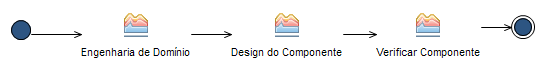
\includegraphics[scale=0.8]{./img/visaogeral.png}
 % matrixargseg.png: 296x162 pixel, 100dpi, 7.52x4.11 cm, bb=0 0 213 117
 %\caption{Estágio desenvolvimento de jogos ~\cite{fullerton2008game}}
\caption{Visão Geral \textit{\ac{gahme} Process}}
%  \caption{Estágio desenvolvimento de jogos}
 \label{fig:visaogeral}
\end{figure}

A Visão Geral do processo (\ref{fig:visaogeral}), contempla duas fases distintas  com responsabilidades bem definidas. 
	\begin{enumerate}
		\item \textbf{Viabilidade:} A primeira fase deverá ser realizado um estudo sobre o público alvo, sintomas a serem monitorados, técnicas e tecnologias que permitam o monitoramento e a viabilidade de realizar o monitoramento dos dados de saúde por intermédio dos jogos eletrônicos.		
		\item \textbf{Desenvolvimento:} A segunda fase utilizará os artefatos de software produzidos durante a primeira fase do processo para desenvolver um jogo eletrônico que permita realizar o monitoramento dos dados de saúde. No final da fase deverá ser realizada uma pesquisa com o público alvo do sistema para comprovar a eficácia do monitoramento.
	\end{enumerate}


\subsection{Viabilidade}\label{sec:viabilidade}
A fase de Viabilidade, terá como papéis principais para a execução das atividades o \textit{Game Health Designer} e o \textit{Profissional de Saúde}. Esses perfis deverão fazer uma análise de viabilidade do monitoramento durante a iteração de \textbf{Iniciação}. Terminada essa iteração, o \textit{Game Designer} irá elaborar cenários de jogos que permitam o monitoramento com a participação do Engenheiro de \textit{Software} que irá implementar protótipos de jogos para testar a abordagem. 

\begin{figure}
 \centering
 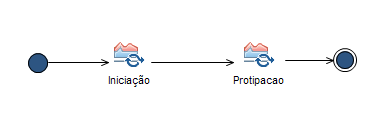
\includegraphics[scale=0.8]{./img/fase-viabilidade.png}
 % matrixargseg.png: 296x162 pixel, 100dpi, 7.52x4.11 cm, bb=0 0 213 117
 %\caption{Estágio desenvolvimento de jogos ~\cite{fullerton2008game}}
\caption{Fase Viabilidade do \textit{GAHME Process}}
%  \caption{Estágio desenvolvimento de jogos}
 \label{fig:faseviabilidade}
\end{figure}

\begin{enumerate}
	\item \textbf{Viabilidade:} Essa iteração será responsável em definir o público alvo do jogo, identificando o tamanho da população beneficiada com o objetivo de avaliar o impacto do desenvolvimento do jogo. Será também responsabilidade desta fase a avaliação dos sintomas possíveis de serem monitorados bem como a existência de sensores que possibilitem o seu monitoramento. O término da fase será um estudo geral da viabilidade de monitoramento dos sintomas através dos jogos eletrônicos.
	\item \textbf{Prototipação:} Nessa iteração serão definidas as tecnologias utilizadas para o desenvolvimento do jogo (\textit{engine} de jogos}) e testar a integração dos sensores dentro da \textit{engine}. Na prototipação deverão ser elaborados cenários de jogos que permitam o monitoramento de dados. E por fim desenvolver protótipos como artefatos de entrada para a elaboração de um artefato que defina as ações que os jogadores deverão realizar e que permita identificar os sintomas monitorados (\textit{GAHME Actions Guideline}).
\end{enumerate}

\subsection{Desenvolvimento}
A fase de Desenvolvimento terá como papéis principais para a execução das atividades o \textit{Game Designer} e o Engenheiro de \textit{Software} resultado final o jogo desenvolvido e comprovação da eficácia do jogo no monitoramento dos dados de saúde. 

\begin{figure}
 \centering
 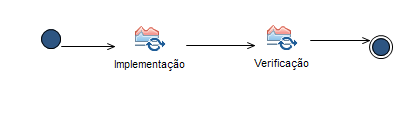
\includegraphics[scale=0.8]{./img/fase-desenvolvimento.png}
 % matrixargseg.png: 296x162 pixel, 100dpi, 7.52x4.11 cm, bb=0 0 213 117
 %\caption{Estágio desenvolvimento de jogos ~\cite{fullerton2008game}}
\caption{Fase Desenvolvimento do \textit{GAHME Process}}
%  \caption{Estágio desenvolvimento de jogos}
 \label{fig:fasedesenvolvimento}
\end{figure}

\begin{enumerate}
	\item \textbf{Desenvolvimento:} A iteração de implementação será bem semelhante a uma fase de produção de um jogo tradicional ~\cite{fullerton2008game}, tendo como produto final da fase o jogo desenvolvido. Contudo, o \textit{Game Design} deverá levar em consideração as ações do jogador que permitem monitoramento (\textit{GAHME Actions Guideline}). No término desta fase, o jogo deverá ser testado com o objetivo de identificar se os mecanismos de captura de dados de saúde do jogo foram desenvolvidos corretamente.
	\item \textbf{Verificação:} 	O desenvolvimento de um jogo por si só é uma tarefa multidisciplinar ~\cite{fullerton2008game} e esta quando aplicada num contexto de saúde necessita de mecanismos para verificar a eficácia da abordagem adotada ~\cite{kato12}. Nessa fase, a proposta do jogo deverá ser submetida para a avaliação do conselho de ética médica, para que possa ser testado com seres humanos e verificar se os sintomas monitorados foram corretamente identificados.
\end{enumerate}


\section{Iteração: Prototipação}
O objetivo desta iteração é desenvolver um protótipo que permita capturar dados de saúde e ao término desta iteração deverá ser elaborado o \textit{GAHME Actions Guideline} (Seção \ref{subsec:game_actions_guide}) que conterá as ações executadas pelo jogador que possam ser monitoráveis e que venham a ser utilizadas pelo \textit{Game Designer} durante a fase de Desenvolvimento. 

Alinhar a jogabilidade e a possibilidade de monitoramento frequente dos dados de saúde não é uma tarefa trivial. Pois deve ser levado em consideração o uso dos dispositivos e pensar na execução de movimentos ou ações que permitam esse monitoramento. Para propor um jogo com monitoramento de dados de saúde deve ser realizado um estudo sobre quais os movimentos e ações que o usuário deve executar. De posse dessas ações, deve ser desenvolvidos protótipos que permitam testar a execução dessas atividades e capturar os dados com o objetivo de estudar mecanismos que permitam identificar esses sintomas conforme os trabalhos já existentes e que possuem tal propósito ~\cite{Ballegaard:2008:HEL:1357054.1357336,albanese2012,bachlin_wearable_2010,visionbased2009,patel_monitoring_2009}. 

\begin{figure}
 \centering
 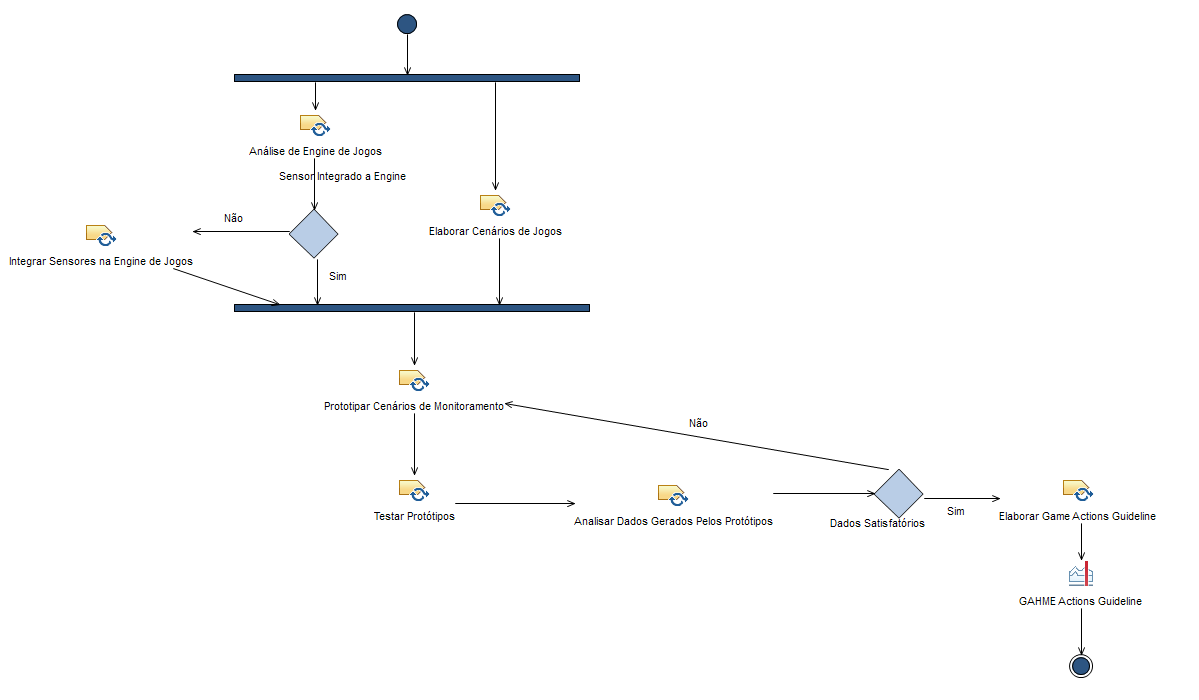
\includegraphics[scale=0.55]{./img/prototipacao.png}
 % matrixargseg.png: 296x162 pixel, 100dpi, 7.52x4.11 cm, bb=0 0 213 117
 %\caption{Estágio desenvolvimento de jogos ~\cite{fullerton2008game}}
\caption{Iteração: Prototipação do \textit{GAHME Process}}
%  \caption{Estágio desenvolvimento de jogos}
 \label{fig:prototipaccao}
\end{figure}

\subsection{Análise de \textit{Engine} de Jogos}
Caso a equipe de desenvolvimento não tenha conhecimento ou experiência sobre uma \textit{engine} de jogos que atendam as necessidades do jogo para monitoramento de dados de saúde, o Engenheiro de \textit{Software} irá analisar as \textit{engine} de jogos existentes e os mecanismos que permitam integrar essa \textit{engine} com os sensores utilizados no jogo.

\subsection{Integrar Sensores à Engine de Jogos}
O Engenheiro de \textit{Software} deve verificar os mecanismos de integrar os sensores que permitem monitoramento dos dados de saúde dentro da \textit{engine} de jogos selecionada na atividade de Análise de \textit{Engine} de Jogos. Alguns sensores como o por exemplo acelerômetro do celular já possuem suporte nativo dentro das \textit{engine} de jogos para esses dispositivos. Outros sensores como o MS-Kinnect ~\cite{kinnect2013} que é uma câmera que permite capturar os movimentos do corpo, necessitam da intalação de \text{Device Drivers} e \textit{plugins} de software a serem instalados dentro da \textit{engine} para permitir a integração. 

Como referência a essa atividade podemos citar o trabalho de mestrado de Santos Jr. ~\cite{antonio2013} que criou um arcabouço de software para monitoramento de dados de saúde com essas tecnologias e fez a integração da \texit{engine} de jogo com sensores que permitem a captura de dados de saúde.

\section{Iteração: Desenvolvimento}
\begin{figure}
 \centering
 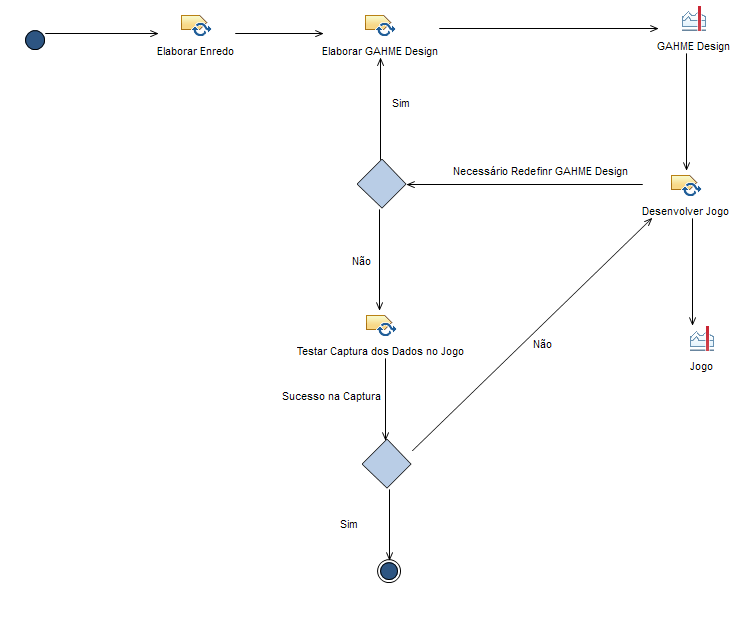
\includegraphics[scale=0.55]{./img/desenvolvimento.png}
 % matrixargseg.png: 296x162 pixel, 100dpi, 7.52x4.11 cm, bb=0 0 213 117
 %\caption{Estágio desenvolvimento de jogos ~\cite{fullerton2008game}}
\caption{Iteração: Desenvolvimento do \textit{GAHME Process}}
%  \caption{Estágio desenvolvimento de jogos}
 \label{fig:desenvolvimento}
\end{figure}

\subsection{Atividade: Elaborar \textit{GAHME Design}}
De posse dos movimentos e da captura dos dados descritos no \textit{Game Action Guideline} será elaborado um \textit{game design} que permita executar esses movimentos em um jogo eletrônico desenvolvido com o objetivo de entreter o usuário ~\cite{sweetser2005-gameflow} e que possua os mecanismos de monitoramento dos dados de saúde embutidos. Para a execução desta atividade deve ser levado em consideração que para a elaboração de um \textit{game design} é necessário um processo iterativo, que precisa ser: prototipado, testado e refinado continuamente até ser concluído ~\cite{brathwaite2009challenges}.

%Os movimentos não podem ser repetitivos pois, levaria o usuário jogar por um curto período e como consequência abandonaria o monitoramento ~\cite{Suhonen:2008:SFE:1457199.1457204}. 



 

%\subsection{Engenheiro de Software}
%Esse papel é responsável por desenvolver o sistema. Os engenheiros de
%software devem utilizar como entrada o \useacronym{DER} gerado pelos engenheiros de requisitos. É
%de extrema importância que os engenheiros de software entendam o
%\useacronym{DER} para que o produto desenvolvido esteja de acordo com sua
%especificação.
%
%\textbf{Habilidades}
%
%Para desempenhar este papel é necessário que o integrante tenha o
%perfil com as  seguintes habilidades:
%
%\begin{compactenum}
    %\item Definir e criar soluções técnicas através das tecnologias utilizadas no projeto.
    %\item Identificar e construir casos de teste que venham cobrir o
%comportamento requerido pelos componentes do sistema.
    %\item Comunicar e repassar a arquitetura da aplicação para os
    %demais integrantes.
%\end{compactenum}
%
%\textbf{Abordagens de Atribuição}
%Mesmo em equipes pequenas, os indivíduos devem trabalhar em grupo no
%desenvolvimento de soluções técnicas.
%
%Cada integrante pode executar tarefas especificas de acordo com suas
%habilidades, porém é desejável que as demais tecnologias utilizadas
%no projeto sejam do conhecimento de todos, para que haja uma maior
%troca de auxilio técnico entre os integrantes.




